\documentclass[aspectratio=169]{beamer}

\usepackage[T1]{fontenc}
\usepackage[utf8]{inputenc}
\usepackage[english]{babel}

\usepackage{amsmath, amssymb, bm, mathtools}
\usepackage{hyperref}

\setbeamertemplate{navigation symbols}{}
\setbeamertemplate{footline}[frame number]

\title{Variational Autoencoders (VAE)}
\subtitle{Full detailed slide deck from the page content before “Обзор статей” (images omitted)}
\author{}
\date{}

% ---------- Notation ----------
\newcommand{\E}{\mathbb{E}}
\newcommand{\Var}{\mathrm{Var}}
\newcommand{\KL}{D_{\mathrm{KL}}}
\newcommand{\cN}{\mathcal{N}}
\newcommand{\cL}{\mathcal{L}}
\newcommand{\R}{\mathbb{R}}

\newcommand{\diag}{\mathrm{diag}}
\newcommand{\tr}{\mathrm{tr}}

\begin{document}

%==================================================
\begin{frame}{What is the problem? Generative modeling}
\begin{itemize}
  \item Data: $D=\{x_i\}_{i=1}^N$, where $x \in \mathcal{X}$ is high-dimensional (e.g., images).
  \item Assume $x_i \sim p_{\text{data}}(x)$.
  \item Goal: learn a probabilistic model $p_\theta(x)$ that approximates $p_{\text{data}}(x)$ and can generate new samples.
  \item Classical objective: maximum likelihood estimation (MLE).
\end{itemize}
\end{frame}

%==================================================
\begin{frame}{Maximum likelihood objective}
\[
\theta^\star \in \arg\max_\theta \sum_{i=1}^N \log p_\theta(x_i).
\]
Equivalently (up to constants), minimize negative log-likelihood:
\[
\min_\theta \; -\frac{1}{N}\sum_{i=1}^N \log p_\theta(x_i).
\]
For expressive models, directly specifying $p_\theta(x)$ is hard; latent-variable models provide a structured approach.
\end{frame}

%==================================================
\begin{frame}{Latent-variable generative models: idea}
Introduce latent variables $z \in \mathcal{Z}$ (typically lower-dimensional):
\[
z \sim p_\theta(z), \qquad x \sim p_\theta(x\mid z).
\]
Joint distribution:
\[
p_\theta(x,z)=p_\theta(x\mid z)\,p_\theta(z).
\]
Marginal likelihood (the model for data):
\[
p_\theta(x)=\int p_\theta(x\mid z)\,p_\theta(z)\,dz.
\]
\begin{itemize}
  \item $p_\theta(z)$: prior over latent space.
  \item $p_\theta(x\mid z)$: decoder / generative conditional distribution.
\end{itemize}
\end{frame}

%==================================================
\begin{frame}{Why latent variables help}
\begin{itemize}
  \item High-dimensional $x$ can be generated from lower-dimensional factors $z$.
  \item Complex, multimodal distributions over $x$ can arise from simple priors over $z$.
  \item Latent space is often smoother and more interpretable (interpolation, clustering, traversals).
\end{itemize}

{\centering
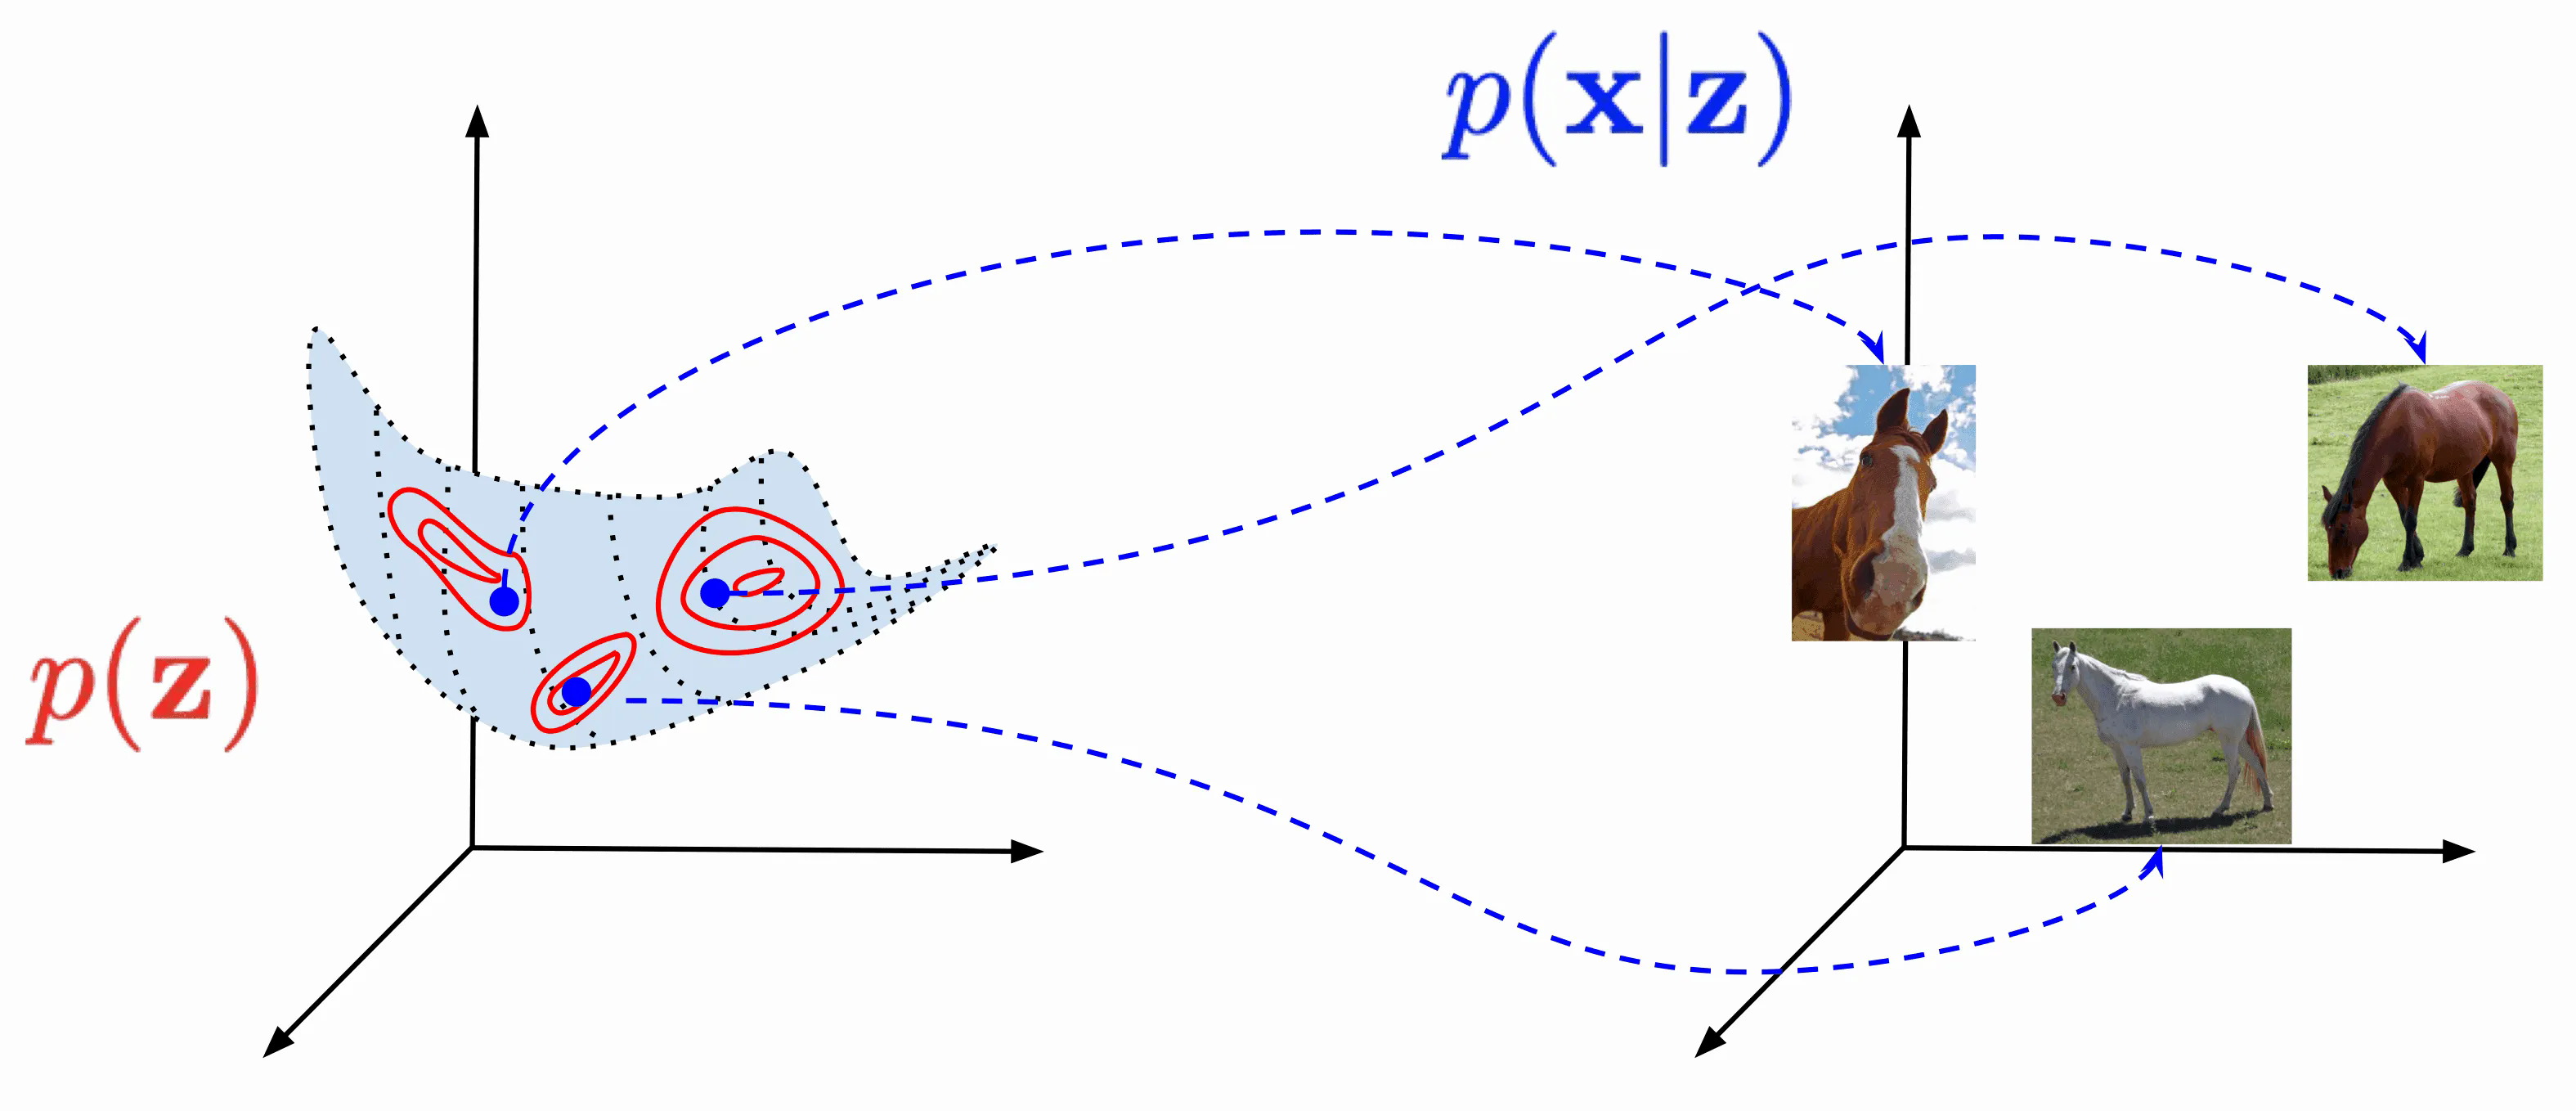
\includegraphics[width=0.80\linewidth]{images/kon.png}\par}

\end{frame}

%==================================================
\begin{frame}{Naive Monte Carlo approximation}
Since
\[
p_\theta(x) = \E_{z\sim p_\theta(z)}\big[p_\theta(x\mid z)\big],
\]
a naive estimator is:
\[
p_\theta(x)\approx \frac{1}{K}\sum_{k=1}^K p_\theta(x\mid z_k), \qquad z_k\sim p_\theta(z).
\]
Problem:
\begin{itemize}
  \item If $p_\theta(x\mid z)$ is sharply peaked, most $z_k$ contribute almost nothing.
  \item Accurate Monte Carlo may require enormous $K$.
\end{itemize}

{\centering
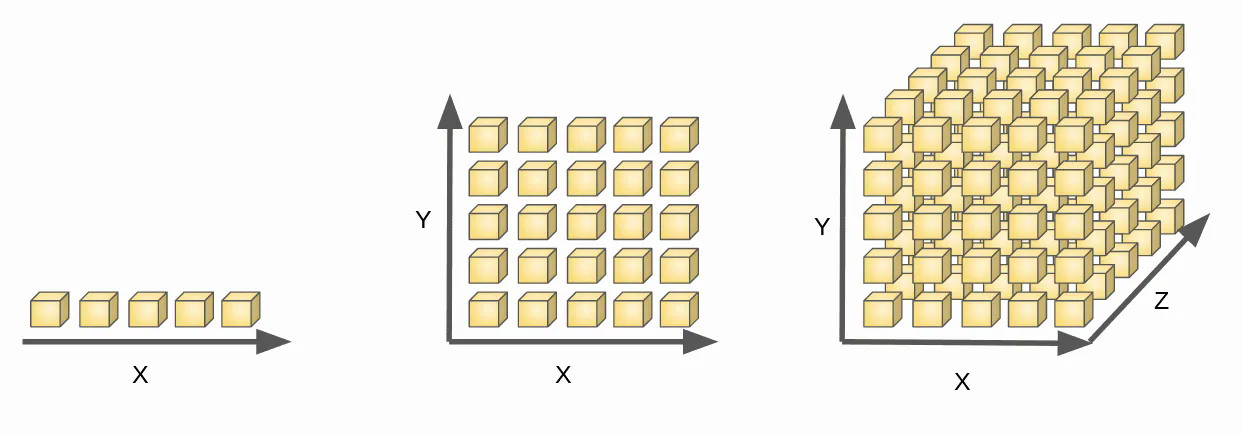
\includegraphics[width=0.80\linewidth]{images/curse_of_dimensionality.png}
\par}

\end{frame}

%==================================================
\begin{frame}{Importance sampling viewpoint}
Rewrite the marginal likelihood using any proposal $q(z\mid x)$:
\[
p_\theta(x)=\int p_\theta(x\mid z)p_\theta(z)\,dz
=\int p_\theta(x\mid z)\frac{p_\theta(z)}{q(z\mid x)}\,q(z\mid x)\,dz.
\]
Hence:
\[
p_\theta(x)=\E_{z\sim q(z\mid x)}\!\left[p_\theta(x\mid z)\frac{p_\theta(z)}{q(z\mid x)}\right].
\]
Monte Carlo estimator:
\[
p_\theta(x)\approx \frac{1}{K}\sum_{k=1}^K p_\theta(x\mid z_k)\frac{p_\theta(z_k)}{q(z_k\mid x)},
\quad z_k\sim q(z\mid x).
\]
If $q(z\mid x)$ concentrates where $p_\theta(x\mid z)$ is large, estimation improves.
\end{frame}

%==================================================
\begin{frame}{ELBO: evidence lower bound}
Start from:
\[
\log p_\theta(x)=\log\int p_\theta(x,z)\,dz.
\]
Multiply and divide by $q_\phi(z\mid x)$:
\[
\log p_\theta(x)
=\log\int q_\phi(z\mid x)\frac{p_\theta(x,z)}{q_\phi(z\mid x)}\,dz
=\log \E_{q_\phi(z\mid x)}\!\left[\frac{p_\theta(x,z)}{q_\phi(z\mid x)}\right].
\]
By Jensen’s inequality:
\[
\log p_\theta(x)\ge \E_{q_\phi(z\mid x)}\left[\log p_\theta(x,z)-\log q_\phi(z\mid x)\right].
\]
Define the ELBO:
\[
\cL_{\theta,\phi}(x) \;=\; \E_{q_\phi(z\mid x)}\left[\log p_\theta(x,z)-\log q_\phi(z\mid x)\right].
\]
\end{frame}

%==================================================
\begin{frame}{Standard ELBO decomposition}
Using $p_\theta(x,z)=p_\theta(x\mid z)p_\theta(z)$:
\begin{align*}
\cL_{\theta,\phi}(x)
&= \E_{q_\phi(z\mid x)}\big[\log p_\theta(x\mid z)\big]
+ \E_{q_\phi(z\mid x)}\big[\log p_\theta(z)\big]
- \E_{q_\phi(z\mid x)}\big[\log q_\phi(z\mid x)\big]\\
&= \E_{q_\phi(z\mid x)}\big[\log p_\theta(x\mid z)\big]
- \KL\big(q_\phi(z\mid x)\,\|\,p_\theta(z)\big).
\end{align*}
Two parts:
\begin{itemize}
  \item Reconstruction (data fit): $\E_{q_\phi(z\mid x)}[\log p_\theta(x\mid z)]$.
  \item Regularization: $-\KL(q_\phi(z\mid x)\|p_\theta(z))$.
\end{itemize}
\end{frame}

%==================================================
\begin{frame}{ELBO gap: relation to the true log-likelihood}
A key identity:
\[
\log p_\theta(x)
=
\cL_{\theta,\phi}(x) + \KL\big(q_\phi(z\mid x)\,\|\,p_\theta(z\mid x)\big).
\]
Since KL is nonnegative:
\[
\log p_\theta(x)\ge \cL_{\theta,\phi}(x).
\]
Interpretation:
\begin{itemize}
  \item Maximizing ELBO increases $\log p_\theta(x)$.
  \item At optimum, if $q_\phi(z\mid x)=p_\theta(z\mid x)$, the bound is tight.
\end{itemize}
\end{frame}

%==================================================
\begin{frame}{Training objective over a dataset}
Maximize the sum of ELBOs:
\[
\max_{\theta,\phi} \sum_{i=1}^N \cL_{\theta,\phi}(x_i)
=
\max_{\theta,\phi} \sum_{i=1}^N
\left(
\E_{q_\phi(z\mid x_i)}[\log p_\theta(x_i\mid z)]
-\KL(q_\phi(z\mid x_i)\|p_\theta(z))
\right).
\]
Stochastic optimization uses mini-batches and Monte Carlo estimates of expectations.
\end{frame}

%==================================================
\begin{frame}{Interpretation of ELBO terms (key ideas)}
\begin{itemize}
  \item \textbf{Reconstruction term}:
  \[
  \E_{q_\phi(z\mid x)}[\log p_\theta(x\mid z)]
  \]
  encourages the decoder to make $x$ likely given latents sampled from the encoder.
  \item \textbf{KL regularizer}:
  \[
  \KL\big(q_\phi(z\mid x)\,\|\,p_\theta(z)\big)
  \]
  encourages the encoded distribution to match the prior, which:
  \begin{itemize}
    \item makes sampling $z\sim p(z)$ produce plausible $x$,
    \item prevents arbitrary, disconnected latent codes.
  \end{itemize}
\end{itemize}
\end{frame}

%==================================================
\begin{frame}{VAE architecture: encoder + decoder}
VAE combines:
\begin{itemize}
  \item \textbf{Encoder} (inference network): $q_\phi(z\mid x)$.
  \item \textbf{Decoder} (generative network): $p_\theta(x\mid z)$.
  \item \textbf{Prior}: $p_\theta(z)$ (often fixed as $\cN(0,I)$).
\end{itemize}
This is ``amortized'' inference: one neural network outputs parameters of $q_\phi(z\mid x)$ for any $x$.
\end{frame}

%==================================================
\begin{frame}{The gradient problem: sampling inside the encoder}
We need gradients of
\[
\E_{q_\phi(z\mid x)}[\log p_\theta(x\mid z)]
\]
w.r.t.\ $\phi$.\\[1.0em]

But $z$ is sampled from $q_\phi(z\mid x)$, which depends on $\phi$ (have you ever taken gradient by parameter of distribution??).\\[1.0em]

Naively, $\nabla_\phi \E_{q_\phi}[\cdot]$ is nontrivial (sampling breaks standard backprop).\\[1.0em]

Solution: \textbf{reparameterization trick} for continuous latents (notably Gaussians).
\end{frame}

%==================================================
\begin{frame}{Reparameterization trick (Gaussian case)}
If
\[
q_\phi(z\mid x)=\cN\big(\mu_\phi(x),\diag(\sigma_\phi^2(x))\big),
\]
sample by:
\[
\varepsilon \sim \cN(0,I),
\qquad
z=\mu_\phi(x)+\sigma_\phi(x)\odot \varepsilon.
\]
Then
\[
\E_{z\sim q_\phi(z\mid x)}[f(z)]
=
\E_{\varepsilon\sim \cN(0,I)}\left[f\big(\mu_\phi(x)+\sigma_\phi(x)\odot \varepsilon\big)\right],
\]
which is differentiable w.r.t.\ $\phi$ through $\mu_\phi,\sigma_\phi$.
\end{frame}

%==================================================
\begin{frame}{Monte Carlo estimate of ELBO (per sample)}
With reparameterization, using $K$ noise samples $\varepsilon_k$:
\[
\cL_{\theta,\phi}(x)
=
\E_{\varepsilon\sim \cN(0,I)}\big[\log p_\theta(x\mid z(\varepsilon))\big]
-\KL(q_\phi(z\mid x)\|p(z)),
\]
approximate:
\[
\cL_{\theta,\phi}(x)\approx
\frac{1}{K}\sum_{k=1}^K \log p_\theta\big(x\mid z_k\big)
-\KL(q_\phi(z\mid x)\|p(z)),
\quad z_k=\mu_\phi(x)+\sigma_\phi(x)\odot\varepsilon_k.
\]
Commonly, $K=1$ works well with mini-batches.
\end{frame}

%==================================================
\begin{frame}{Connection to classical autoencoders}
Deterministic autoencoder:
\[
z=f_\phi(x),\qquad \hat{x}=g_\theta(z),
\]
with reconstruction loss (e.g., $\|x-\hat{x}\|^2$).

VAE differences:
\begin{itemize}
  \item encoder outputs a \emph{distribution} $q_\phi(z\mid x)$, not a point,
  \item decoder is probabilistic $p_\theta(x\mid z)$,
  \item KL term shapes $z$ to follow a chosen prior, enabling unconditional sampling.
\end{itemize}
\end{frame}

%==================================================
\begin{frame}{Typical training loop (mini-batch SGD)}
For a mini-batch $\{x_b\}_{b=1}^B$:
\begin{enumerate}
  \item Encoder forward: compute $\mu_b=\mu_\phi(x_b)$ and $\log\sigma_b^2=\log\sigma_\phi^2(x_b)$.
  \item Sample noise: $\varepsilon_b\sim\cN(0,I)$.
  \item Reparameterize: $z_b=\mu_b+\sigma_b\odot\varepsilon_b$.
  \item Decoder forward: compute parameters of $p_\theta(x_b\mid z_b)$.
  \item Compute:
  \[
  \widehat{\cL}=\frac{1}{B}\sum_{b=1}^B \log p_\theta(x_b\mid z_b)
  -\frac{1}{B}\sum_{b=1}^B \KL\big(q_\phi(z\mid x_b)\|p(z)\big).
  \]
  \item Update $\theta,\phi$ by ascending $\widehat{\cL}$ (or descending $-\widehat{\cL}$).
\end{enumerate}
\end{frame}

%==================================================
\begin{frame}{Generation after training}
After training, to generate a new sample:
\[
z \sim p(z)\quad (\text{often } \cN(0,I)),
\qquad
x \sim p_\theta(x\mid z).
\]
\end{frame}

%==================================================
\begin{frame}{Latent space properties (key ideas)}
Because $q_\phi(z\mid x)$ is regularized toward $p(z)$:
\begin{itemize}
  \item nearby points in latent space often decode to semantically similar outputs,
  \item interpolation is meaningful: for $z(t)=(1-t)z_0+t z_1$
  \item latent space can reflect class structure (clusters/regions) when data has discrete modes.
\end{itemize}

{\centering
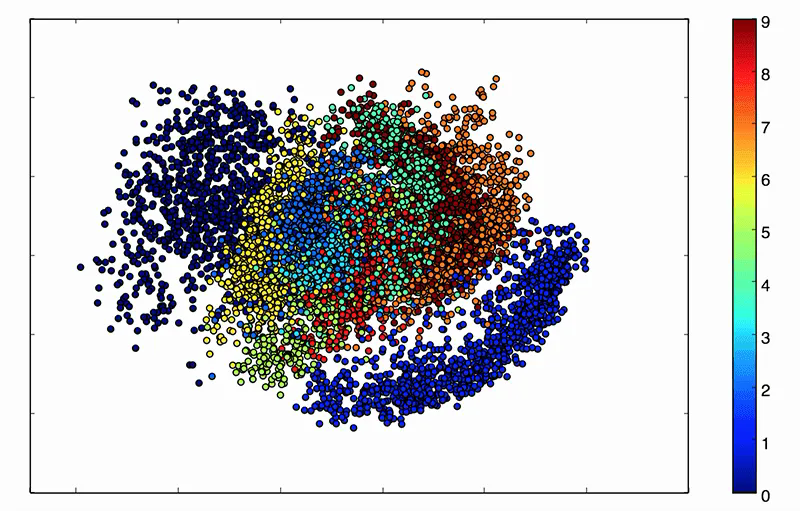
\includegraphics[width=0.60\linewidth]{images/cluster.png}\par}

\end{frame}

%==================================================
\begin{frame}{Manifold}

{\centering
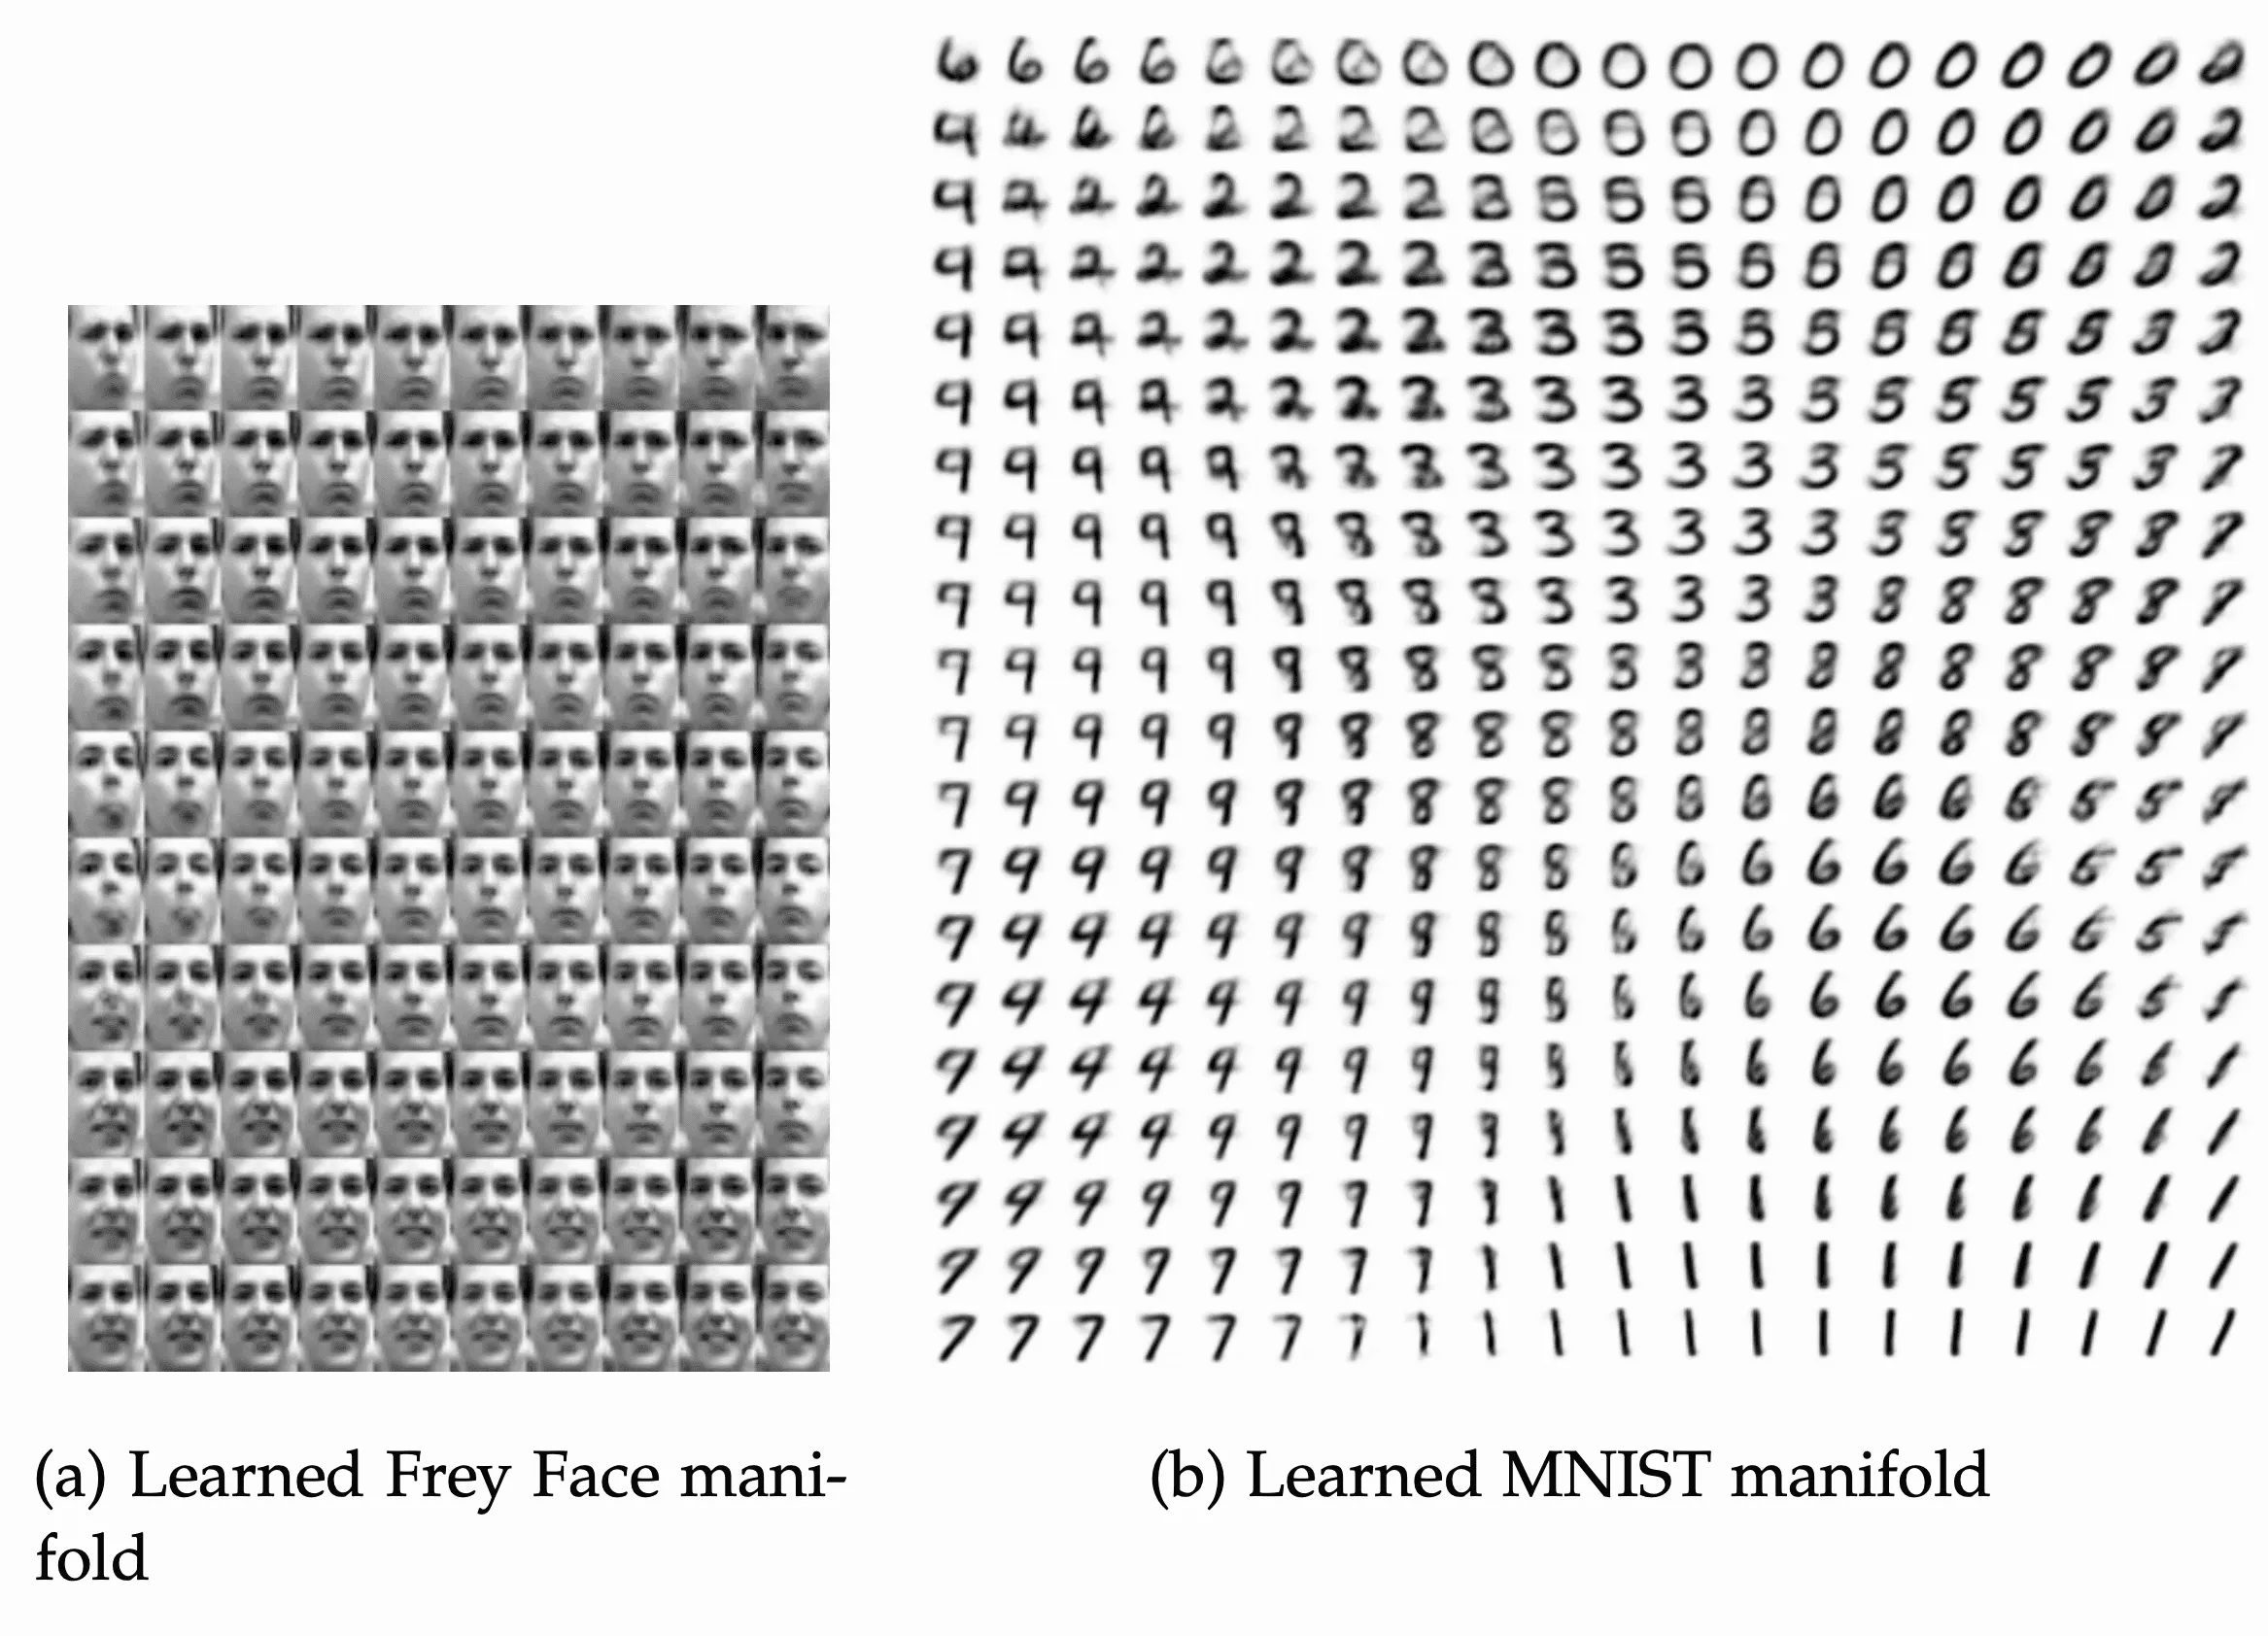
\includegraphics[width=0.80\linewidth]{images/manifold.png}\par}

\end{frame}

%==================================================
\begin{frame}{Why the KL term matters for sampling}
If we trained only reconstruction (like a deterministic autoencoder):
\begin{itemize}
  \item encoded $z$ could occupy an arbitrary set in $\R^M$,
  \item sampling $z\sim \cN(0,I)$ would likely land outside that set,
  \item decoded samples would be garbage.
\end{itemize}
KL regularization enforces:
\[
q_\phi(z\mid x)\approx p(z),
\]
so that sampling from $p(z)$ produces latents similar to those seen during training.
\end{frame}

%==================================================
\begin{frame}{Conditional generation: motivation}
Sometimes we want to generate not from the overall distribution $p(x)$,
but from a conditional distribution $p(x\mid y)$ for some attribute/label $y$:
\begin{itemize}
  \item class label (digits, categories),
  \item style, domain, speaker identity,
  \item any conditioning information available at train/test time.
\end{itemize}
Solution: \textbf{Conditional VAE (CVAE)}.
\end{frame}

%==================================================
\begin{frame}{Conditional VAE: model and inference}
Introduce condition $y$ and define:
\[
p_\theta(z\mid y),\qquad p_\theta(x\mid z,y),\qquad q_\phi(z\mid x,y).
\]
The conditional marginal likelihood:
\[
p_\theta(x\mid y)=\int p_\theta(x\mid z,y)p_\theta(z\mid y)\,dz.
\]
ELBO for CVAE:
\[
\cL_{\theta,\phi}(x,y)
=
\E_{q_\phi(z\mid x,y)}[\log p_\theta(x\mid z,y)]
-\KL\big(q_\phi(z\mid x,y)\,\|\,p_\theta(z\mid y)\big).
\]
\end{frame}

%==================================================
\begin{frame}{CVAE: sampling}
To generate conditioned on $y$:
\[
z \sim p_\theta(z\mid y),\qquad x \sim p_\theta(x\mid z,y).
\]
Common choices:
\begin{itemize}
  \item $p_\theta(z\mid y)=\cN(0,I)$ for all $y$, but feed $y$ only to the decoder and encoder;
  \item or a class-dependent prior $p_\theta(z\mid y)=\cN(\mu_y,\Sigma_y)$ (or NN-parameterized).
\end{itemize}
\end{frame}

\begin{frame}{Why CVAE can separate classes better than a vanilla VAE}
In a \textbf{vanilla VAE}, all data classes share one latent prior: \(p(z)\sim \mathcal{N}(0,I)\).

\vspace{0.6em}
In a \textbf{Conditional VAE (CVAE)}, we condition the prior on the label $y$ and effectively give each class its own latent space:
\[
p(z\mid y)\sim \mathcal{N}(0,I)\qquad \text{for each } y\in\{0,\dots,9\}.
\]

{\centering
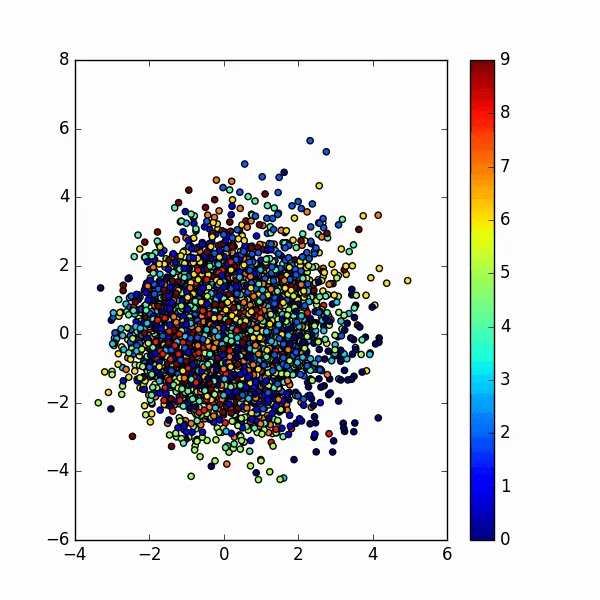
\includegraphics[width=0.40\linewidth]{images/manimanifold.png}\par}

\end{frame}

\begin{frame}{Why CVAE can separate classes better than a vanilla VAE}

As a result, the model does not need to pack all digits into one shared $p(z)$; it can learn \emph{class-specific} latent structure, which often yields cleaner class separation.

\vspace{0.8em}

{\centering
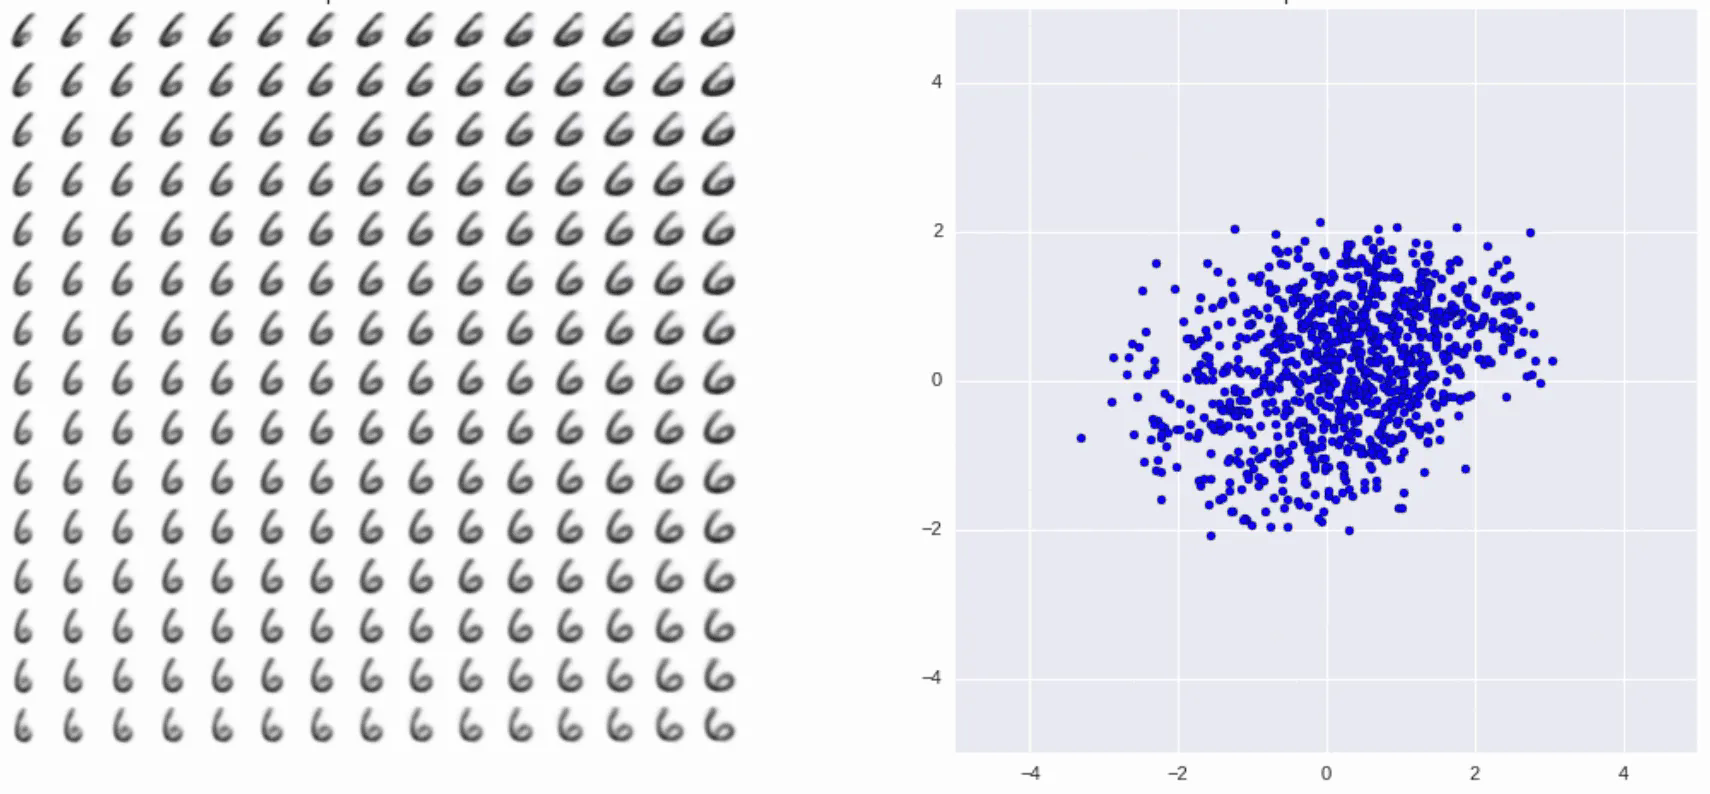
\includegraphics[width=0.80\linewidth]{images/six_manifold.png}\par}

\end{frame}


%==================================================
\begin{frame}{ELBO recap and the full picture}
For (unconditional) VAE:
\[
\log p_\theta(x)
\ge
\underbrace{\E_{q_\phi(z\mid x)}[\log p_\theta(x\mid z)]}_{\text{data fit / reconstruction}}
-
\underbrace{\KL(q_\phi(z\mid x)\|p(z))}_{\text{latent regularization}}.
\]
Training:
\[
\max_{\theta,\phi} \sum_{i=1}^N \cL_{\theta,\phi}(x_i).
\]
After training:
\[
z\sim p(z)\Rightarrow x\sim p_\theta(x\mid z).
\]
\end{frame}

\end{document}
